\chapter{Differnetial analysis of the NN output}
%\chapter{Analysis of the effects of different event features on the neural network output}
\section{Weighted correlations of input features with the NN output}

\subsection{Motivation for calculating correlations}
Correlations between input variables and the neural network's provide an overview of what the NN has "learned". 
They represent which input variables have the strongest influence on the output of the NN. 
The level of influence of any input variable is determined during the training phase of the NN. For example, suppose the value of a specific input variable turns out to be an essential parameter in the discrimination of the signal from the background. 
In that case, this variable will acquire a high correlation after the training process. 
Consequently, highly correlated variables would provide a critical basis to determine which properties of the $tq\gamma$ process help in understanding the photon to top quark coupling.  \\

\subsection{Steps of calculation}

Weighted correlations between two sets of data are calculated by first determining the covariance of these sets. For the covariance, the weighted mean of each set is needed. 
The weighted mean is calculated as follows
\begin{align*}
    m(x;w) &= \frac{\sum_i{w_i x_i}}{\sum_i{ w_i}}
\end{align*}
where $x$ is the given set over which to calculate the mean. In this section, $x$ represents one input feature of a process or the NN output values. The weights of each data point is given by $w$. 
The covariance is then calcuted with the formula 
\begin{align*}
    cov(x,y;w) &= \frac{\sum_i{w_i \cdot (x_i - m(x;w)) \cdot (y_i - m(y;w))}}{\sum_i{w_i}}.
\end{align*}
Here, $y$ stands for the second data set. Finally, the weighted correlation is then determined to be 
\begin{align*}
    corr(x,y;w) &= \frac{cov(x,y;w)}{\sqrt{cov(x,x;w)\cdot cov(y,y;w)}}.
\end{align*}
Thus, the correlation between the values for one input feature $X_\text{input}$ and the NN output values $Y_\text{output}$ with the weights $W$ would be $corr(X_\text{input},Y_\text{output};W)$.

Calculations for the $0\, fj$ region and the $\geq 1\, fj$ region are done separately.  
Every generated event is saved with 110 different features, including the input features, the NN output value and the NN weights. 
At the start, the calculation for variable correlations with the NN output is performed for all events of the same sample.  
Then, all correlations of the background samples are combined. This is done by calculating a weighted mean over all samples. Here, the sum of weights in a sample is used as the new weight for the mean.
Finally, the correlation of measured data is also determined. The final result is a correlation table for the whole background, the $tq\gamma$ process and the measured data in each forward jet region. 
The result of the calculations is visualised and discussed in Section \ref{sec:corrvis}.


\subsection{Visualisations of calculated correlations}
\label{sec:corrvis}
The results of the calculations are listed in Table \ref{tab:corrAll}. This table also contains some correlations of features that are not part of the input of the NN in the given region.  
Figure \ref{fig:corr0fj} and \autoref{fig:corr1fj} display correlations of the input features in order for both forward jet regions respectively. 

\textbf{Spreche über einige variablen und erkläre warum Sie stark oder weniger stark korreliert sind. Dann muss auch ph\_pt angesprochen werden. Anschließend kann fjph\_e mit fj\_e verglichen werden.}

\begin{table}[htbp]
    \centering
    \begin{tabular}{c|c c c|c c c}
        \toprule
        {}&\multicolumn{3}{c}{$0\, fj$ region}&\multicolumn{3}{c}{$\geq 1\, fj$ region}\\
        Event parameter &  Background &  $tq\gamma$ &  Data &  Background &  $tq\gamma$ &  Data \\
        \midrule
        top\_m                            & -0.51 &      0.01 &   0.03 & -0.41 &      0.06 &   0.04 \\ \hline
        Wbsn\_e                           & -0.35 &     -0.02 &   0.00 & -0.38 &      0.00 &  -0.00 \\ \hline
        blep\_m                           & -0.39 &      0.01 &   0.01 & -0.33 &      0.02 &   0.01 \\ \hline
        topph\_ctheta                     & -0.28 &     -0.00 &     & -0.33 &     -0.01 &   0.02 \\ \hline
        transMassWb                      & -0.47 &     -0.00 &     & -0.33 &     -0.02 &  -0.02 \\ \hline
        lep1\_pt                          & -0.36 &        &     & -0.32 &      0.54 &   0.43 \\ \hline
        HT                               & -0.21 &     -0.24 &  -0.35 & -0.30 &     -0.22 &  -0.32 \\ \hline
        met\_met                          & -0.26 &     -0.05 &   0.02 & -0.26 &      0.00 &  -0.01 \\ \hline
        topph\_pt                         & -0.02 &     -0.12 &  -0.14 & -0.18 &     -0.06 &  -0.03 \\ \hline
        blep\_dr                          & -0.15 &     -0.06 &  -0.14 & -0.14 &     -0.05 &  -0.07 \\ \hline
        bph\_pt                           & -0.08 &     -0.03 &   0.02 & -0.13 &      0.00 &   0.02 \\ \hline
        transMassWph                     & -0.17 &      0.00 &  -0.00 & -0.10 &      0.00 &   0.02 \\ \hline
        fjph\_dr                          &  0.00 &      0.18 &   0.19 & -0.06 &      0.14 &   0.15 \\ \hline
        lbj\_pt                           & -0.12 &     -0.32 &  -0.50 & -0.05 &     -0.24 &  -0.42 \\ \hline
        fjph\_deta                        &  0.00 &     -0.36 &  -0.29 & -0.03 &     -0.29 &  -0.33 \\ \hline
        fj\_phi                           & -0.00 &     -0.09 &  -0.08 & -0.03 &     -0.11 &  -0.19 \\ \hline
        lep1\_eta                         &  0.02 &     -0.30 &  -0.37 & -0.02 &     -0.28 &  -0.39 \\ \hline
        met\_phi                          &  0.00 &      0.27 &   0.14 & -0.01 &      0.25 &   0.18 \\ \hline
        lep1\_id                          & -0.16 &     -0.27 &  -0.43 & -0.00 &     -0.20 &  -0.35 \\ \hline
        ph\_eta                           &  0.00 &        &     &  0.00 &      0.45 &   0.22 \\ \hline
        ph\_phi                           & -0.00 &     -0.05 &  -0.09 &  0.01 &     -0.08 &  -0.13 \\ \hline
        fj\_eta                           & -0.00 &        &     &  0.01 &     -0.05 &  -0.01 \\ \hline
        lbj\_phi                          & -0.00 &      0.07 &   0.03 &  0.01 &      0.45 &   0.28 \\ \hline
        lbj\_eta                          &  0.02 &     -0.02 &   0.00 &  0.02 &     -0.16 &  -0.09 \\ \hline
        fjph\_m                           &    &     -0.02 &   0.00 &  0.04 &     -0.16 &  -0.08 \\ \hline
        ph\_pt                            &  0.06 &        &     &  0.08 &      0.29 &   0.14 \\ \hline
        fjph\_ctheta                      &    &      0.25 &   0.15 &  0.08 &      0.12 &   0.12 \\ \hline
        lepph\_dr                         &  0.10 &     -0.03 &  -0.19 &  0.11 &     -0.01 &  -0.14 \\ \hline
        lbj\_tagWeightBin &  0.12 &     -0.16 &  -0.21 &  0.13 &     -0.17 &  -0.25 \\ 
        \_DL1r\_Continuous &&&&&&\\ \hline
        bfj\_m                            &    &      0.02 &  -0.00 &  0.19 &     -0.01 &   0.00 \\ \hline
        bph\_m                            &  0.19 &     -0.20 &  -0.24 &  0.25 &     -0.26 &  -0.34 \\ \hline
        fjph\_e                           &  0.04 &     -0.07 &  -0.13 &  0.27 &     -0.03 &  -0.10 \\ \hline
        fjet\_flag                        &    &     -0.28 &  -0.42 &  0.37 &     -0.19 &  -0.31 \\ \hline
        \bottomrule
        \end{tabular}
    \caption{List of correlations between samples and the NN output in the zero forward jet region as well as samples in the $\geq 1$ forward jet region.}
    \label{tab:corrAll}
\end{table}
\begin{figure}
    \centering
    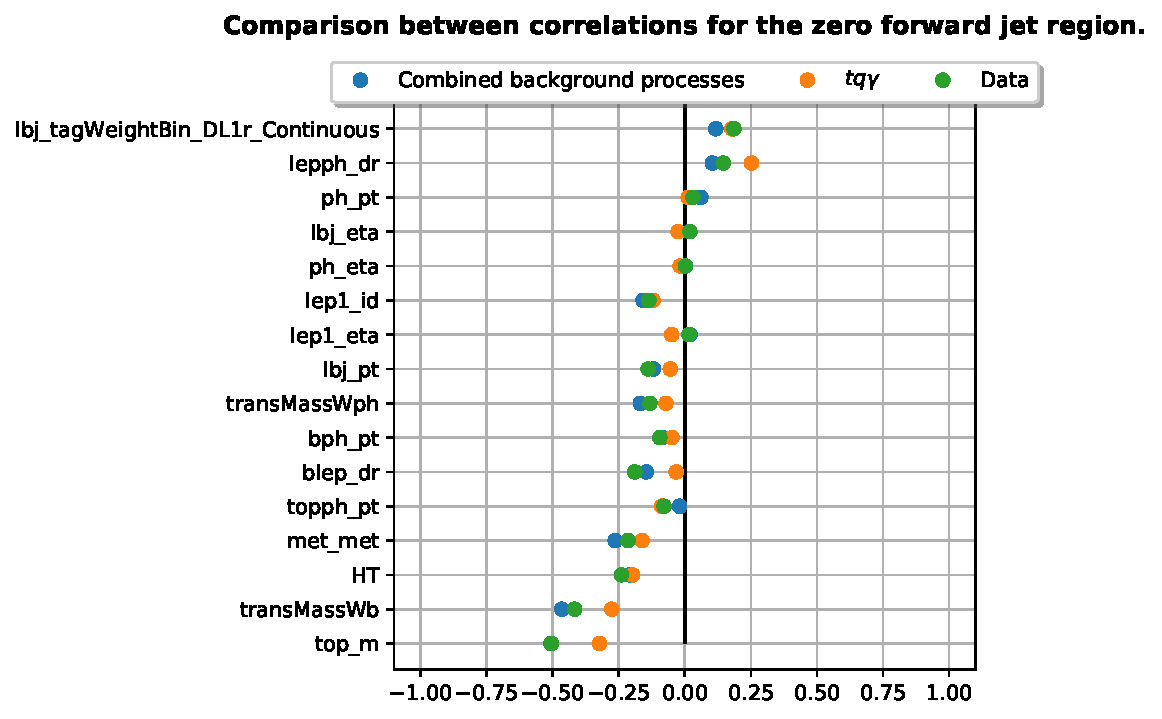
\includegraphics[width=0.7\textwidth]{Plots/corr0fjvariables.pdf}
    \caption{Visualisation of the correlations of input variables with the NN output in the $0\,fj$ region for the background samples, $tq\gamma$ and the measured data.}
    \label{fig:corr0fj}
\end{figure}
\begin{figure}
    \centering
    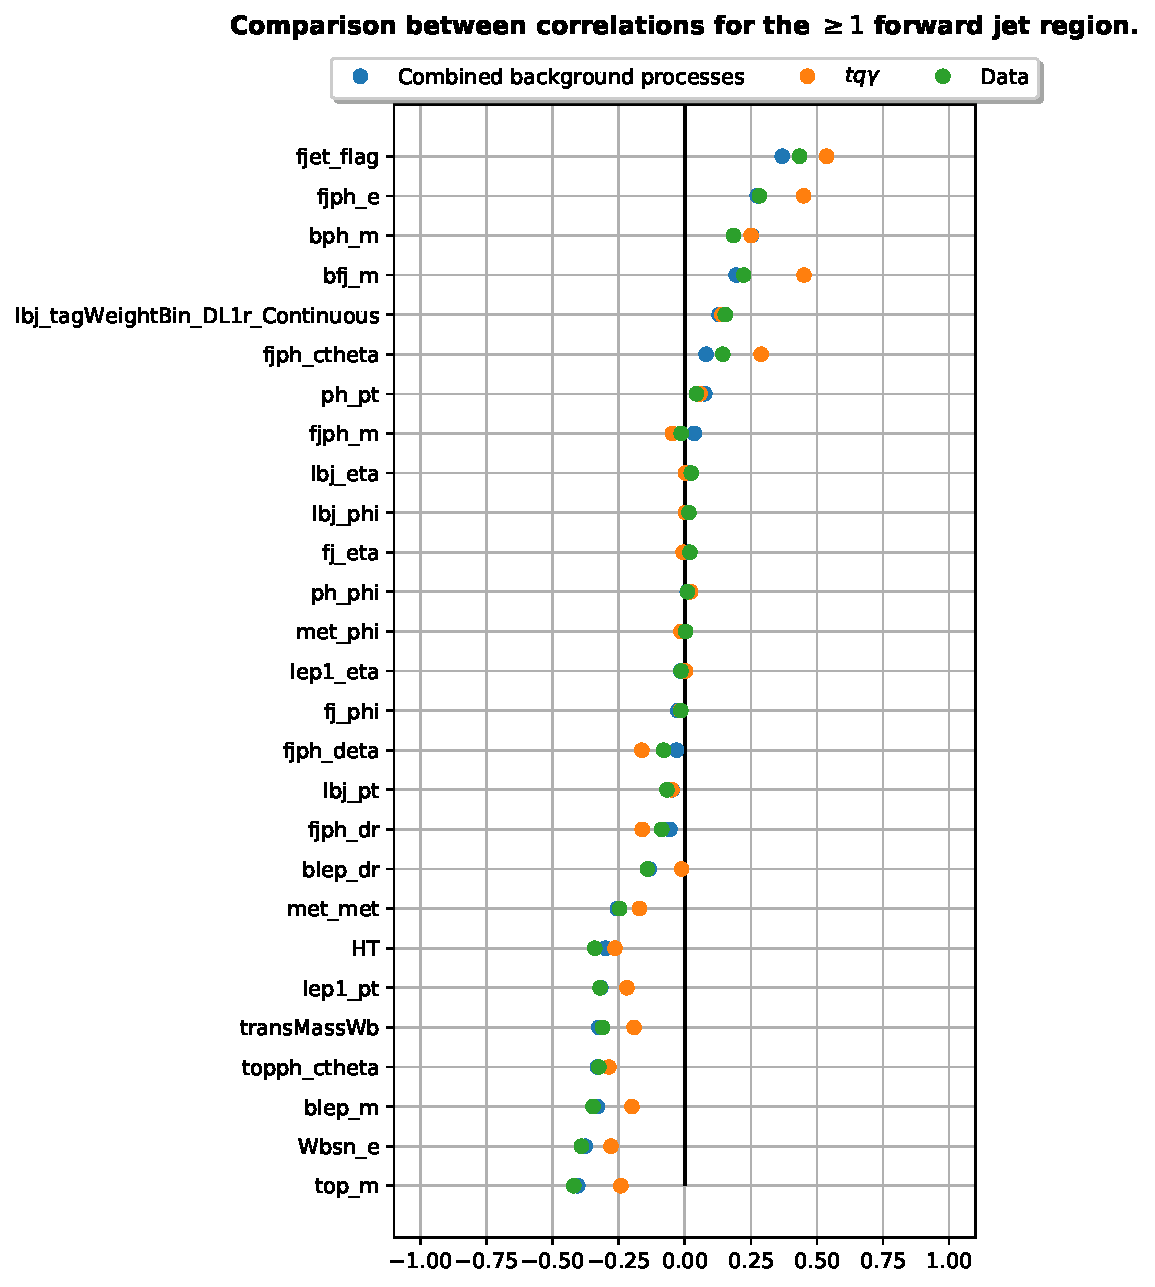
\includegraphics[width=0.7\textwidth]{Plots/corr1fjvariables1.pdf}
    \caption{Visualisation of the correlations of input variables with the NN output in the $\geq 1\,fj$ region for the background samples, $tq\gamma$ and the measured data.}
    \label{fig:corr1fj}
\end{figure} 

\section{NN output distribution dependence on photon \texorpdfstring{$p_T^\gamma$}{pTGamma} and fjet+photon energy \texorpdfstring{$E_{fj\text{+}\gamma}$}{}}
\label{sec:dependence}

In this section, two input variables are chosen to analyse the influence on the NN output further. In the first part of the analysis, an energy region for the input variables is chosen. Then, only events within that energy region are considered. This will be referred to as a "cut" throughout this section. 
After the cut, the distribution of the NN output is plotted to determine any noticeable changes. Additionally, a threshold for the NN output is chosen, and every event above the threshold is considered as a signal. The signal above the threshold must not exceed a statistical error $\frac{N_\text{signal}}{\sqrt{N_\text{signal}}}$ of over $10\%$. 
The composition of events above the threshold is then visualised and discussed. Changes in signal and background compositions are examined. For simplicity, only the $\geq 1$ forward jet region is considered in this analysis.

To compare with the NN output before any cut is applied, the Figure~\ref{fig:full} gives the composition of NN output for two different threshholds. One at $NN = 0.9$ and the other at the highest possible threshhold before the statistical error becomes too high.
\begin{figure}
    \centering
    \begin{subfigure}[b]{0.6\textwidth}
       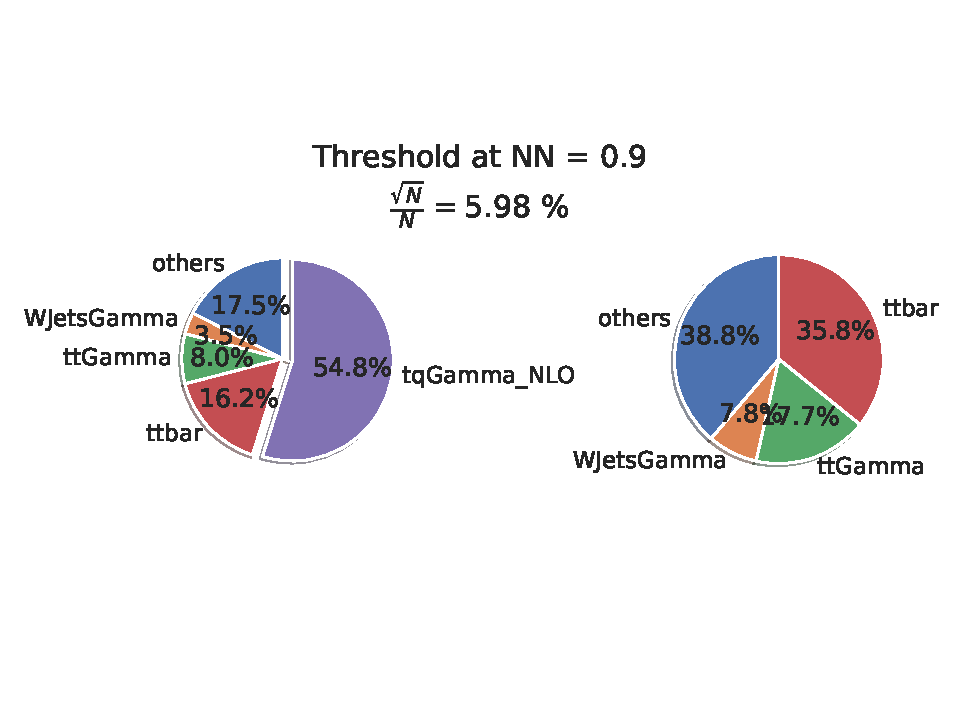
\includegraphics[width=1\linewidth]{Plots/composition9FULL.pdf}
    \end{subfigure}
    
    \begin{subfigure}[b]{0.6\textwidth}
       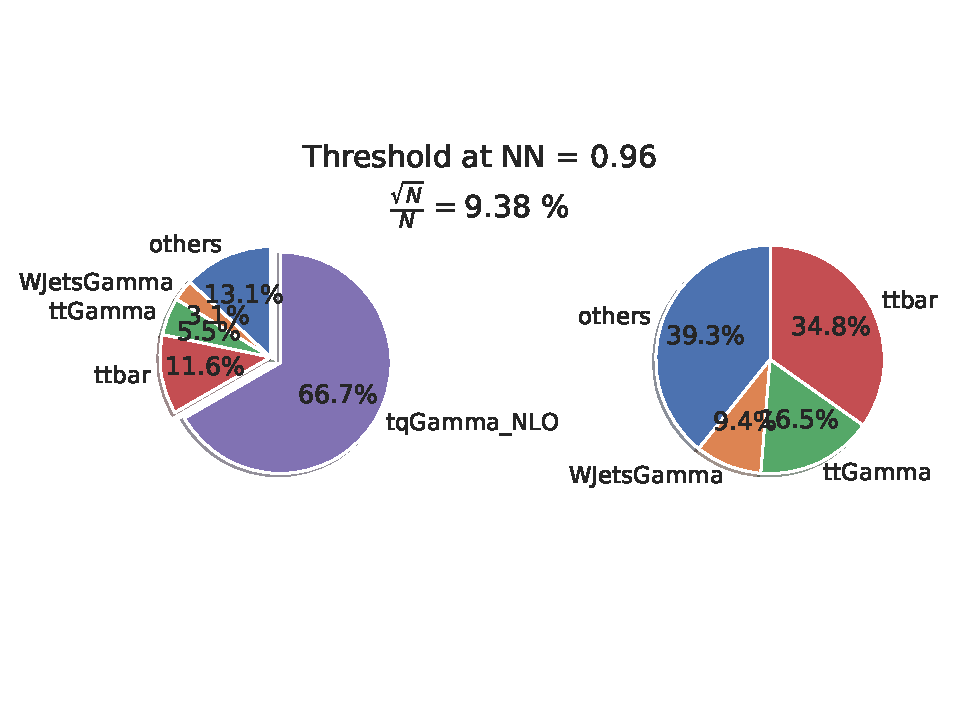
\includegraphics[width=1\linewidth]{Plots/compositionTenFULL.pdf}
    \end{subfigure}
    \caption{Composition of NN output for two different threshholds without any cuts applied. The right pie chart gives the composition without of the background.}
    \label{fig:full}
\end{figure}

The first input variable that is to be analysed is the transverse momentum of the photon $p_T^\gamma$. As the $tq\gamma$ process is sensitive to the top quark to photon coupling, analysing the output dependence of the momentum of the photon provides a good way to test this prediction. 
Results from \autoref{sec:corrvis} give a low correlation of $p_T^\gamma$ at around $15.5\%$ in the $\geq 1\, fj$ region. The dependence of the NN output on $p_T^\gamma$ is therefore found not to be significant. The composition still remains of interest. 

The distribution of $p_T^\gamma$ is shown in \autoref{fig:ph_pt}. 

\begin{figure}[htbp]
    \centering
    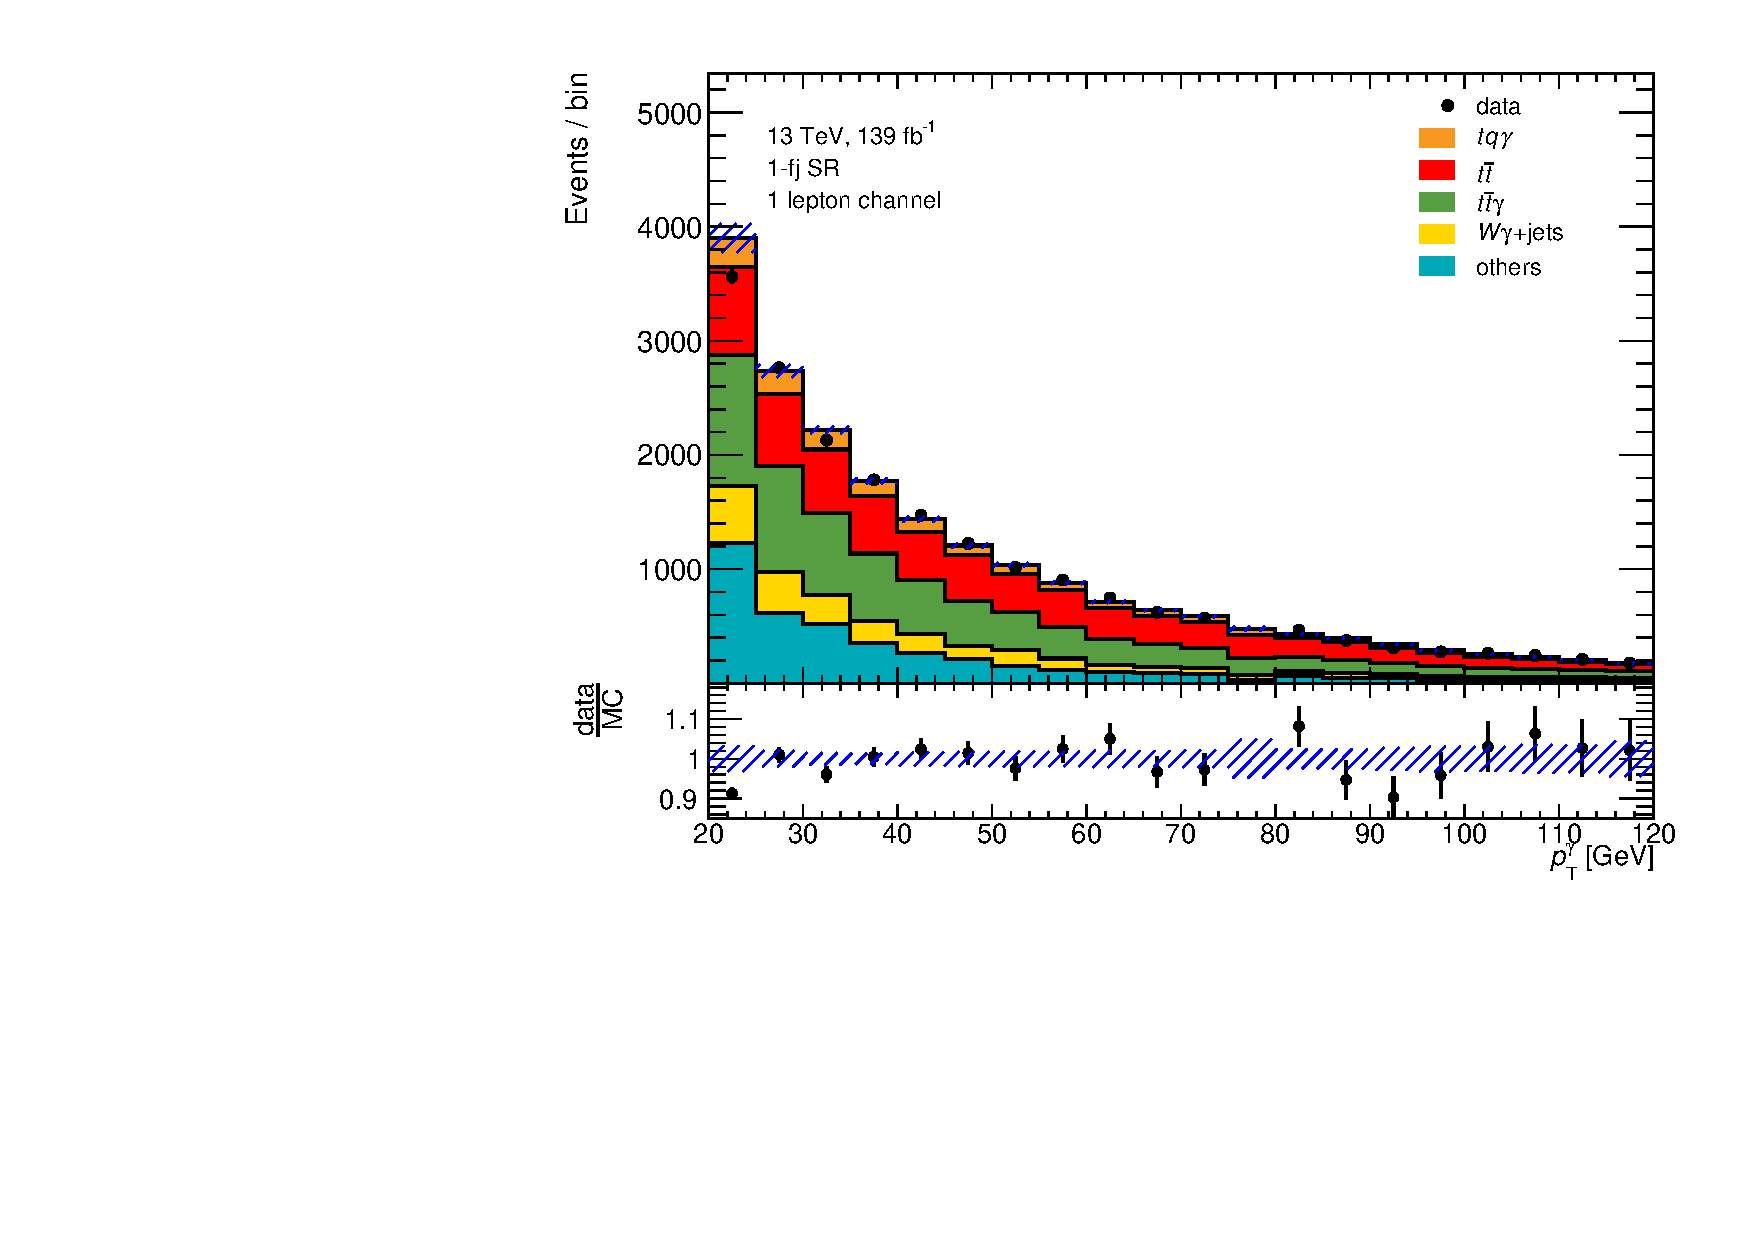
\includegraphics[width=0.6\textwidth]{Plots/ph_pt.pdf}
    \caption{Distribution of the transverse momentum of the photon $p_T^\gamma$.}
    \label{fig:ph_pt}
\end{figure}

With the help of the distribution it is chosen to cut $p_T^\gamma$ at $40\,\si{\giga\electronvolt}$. The positive correlation predicts that higher $p_T^\gamma$ result in a better signal-background discrimination in the NN output. 
The NN output distribution for events with $p_T^\gamma \geq 40\,\si{\giga\electronvolt}$ is displayed in \autoref{fig:outputA40ph}. The composition after two different threshholds is shown in \autoref{fig:phptA40}.

\begin{figure}
    \centering
    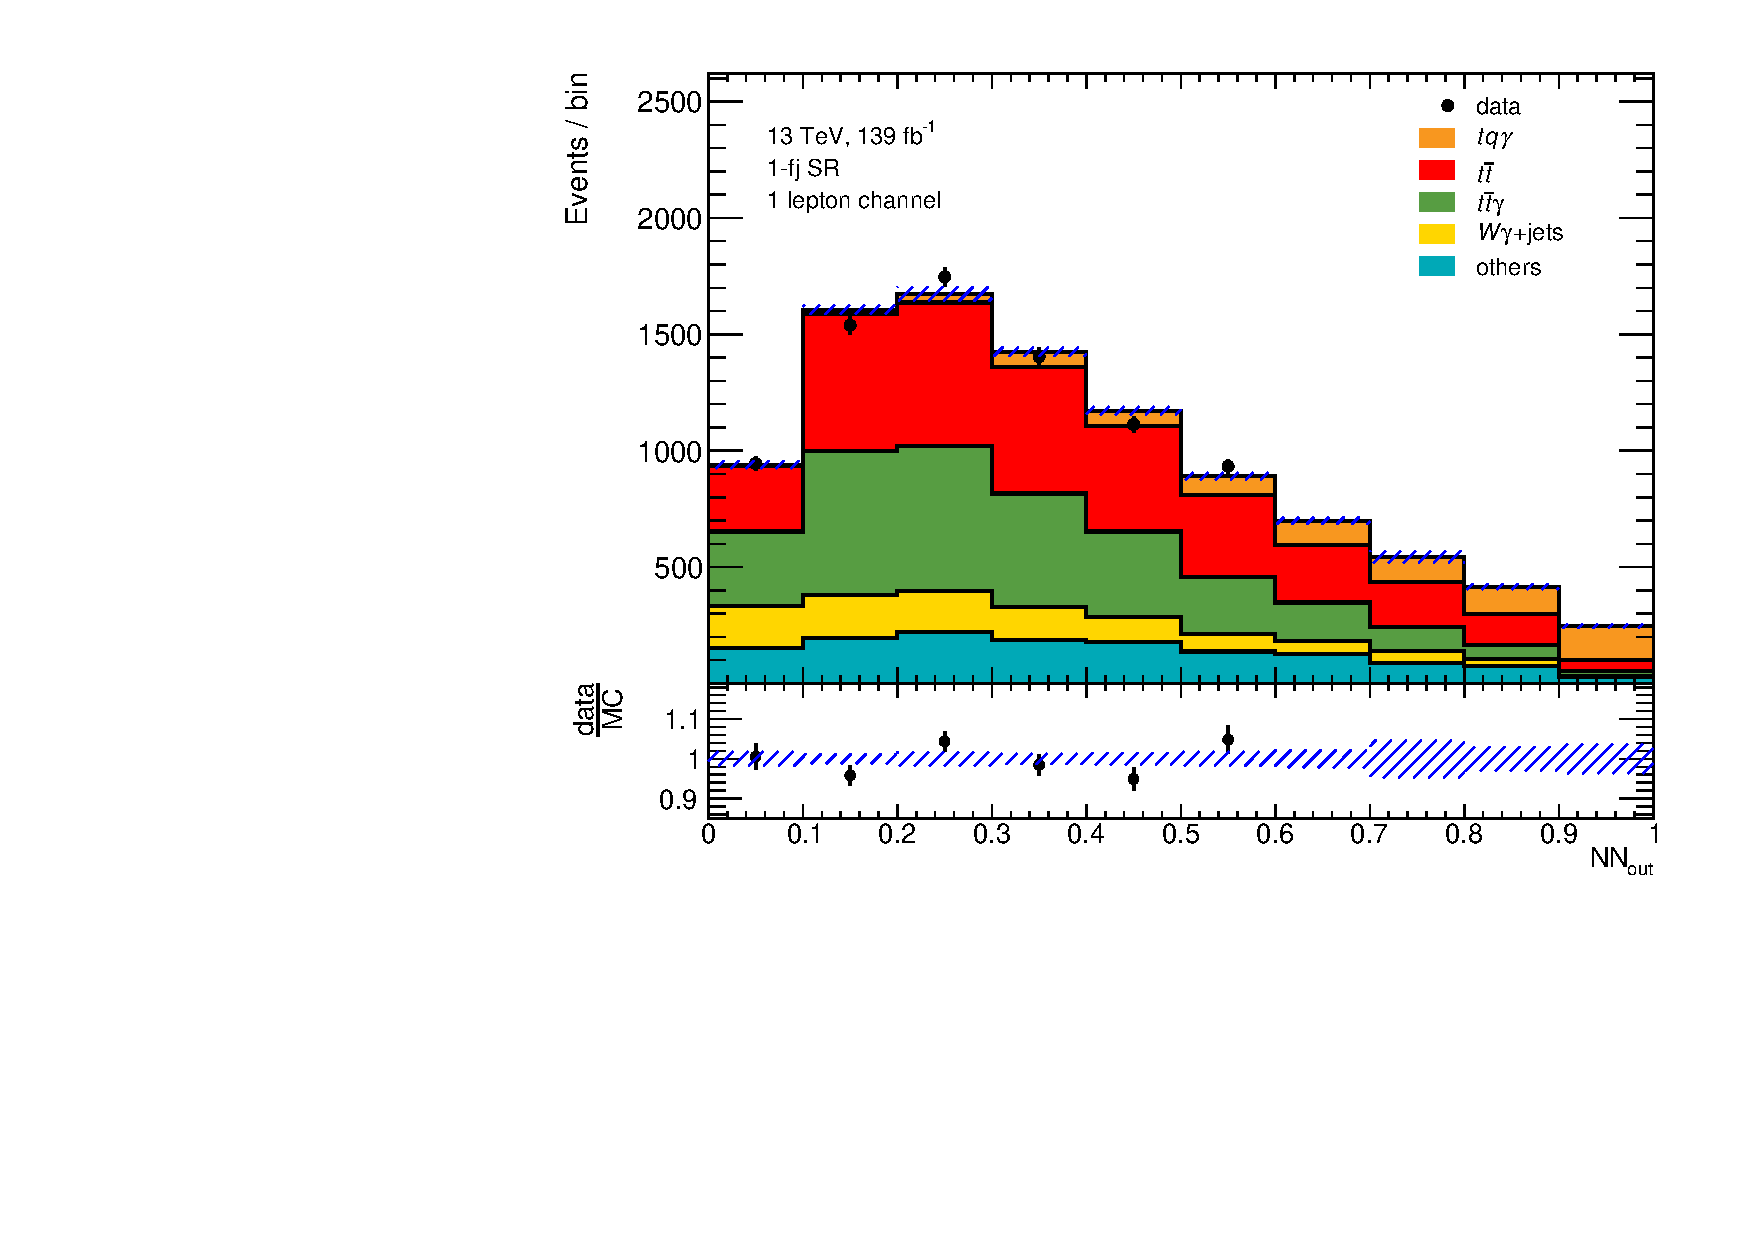
\includegraphics[width=0.7\textwidth]{Plots/NN_out_mixphA40.pdf}
    \caption{NN output distribution for the $p_T^\gamma \geq 40\,\si{\giga\electronvolt}$ region.}
    \label{fig:outputA40ph}
\end{figure} 

\begin{figure}
    \centering
    \begin{subfigure}[b]{0.6\textwidth}
       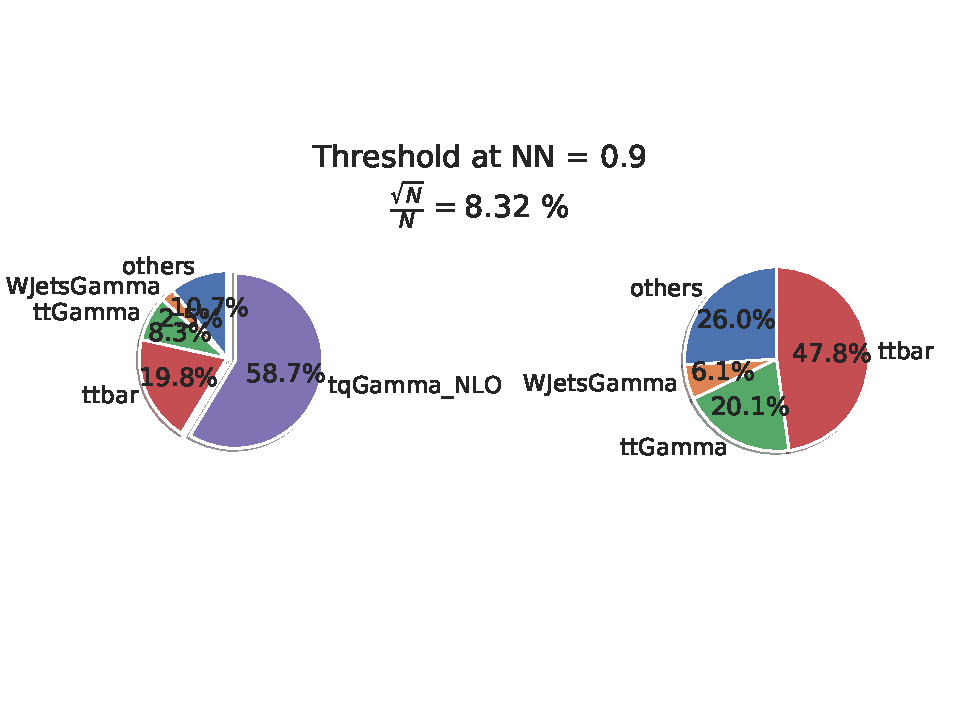
\includegraphics[width=1\linewidth]{Plots/composition9phA40.pdf}
    \end{subfigure}
    
    \begin{subfigure}[b]{0.6\textwidth}
       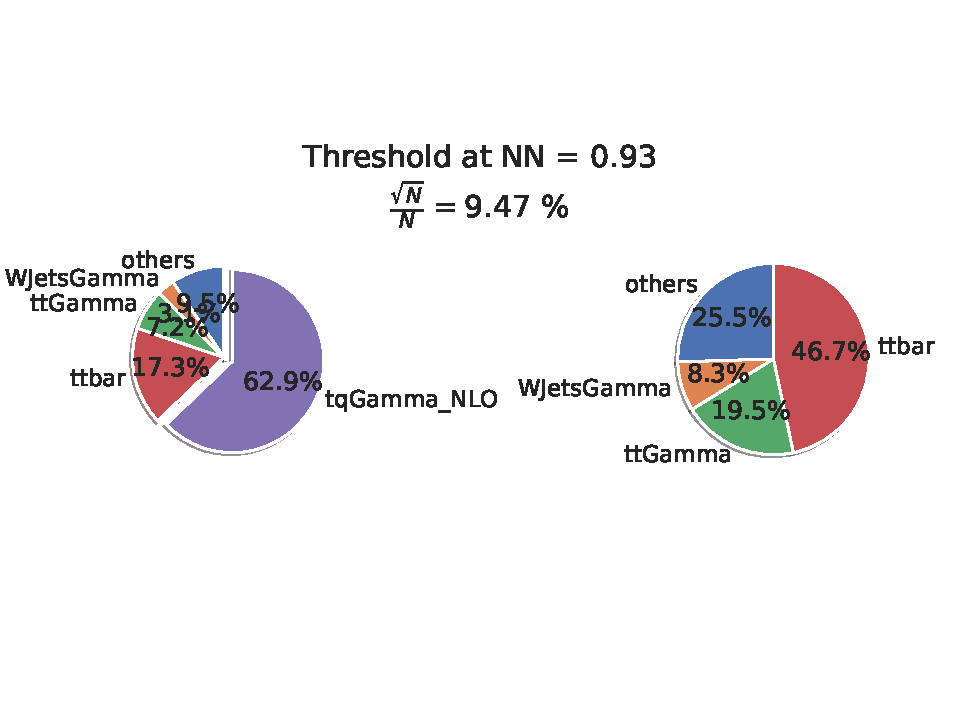
\includegraphics[width=1\linewidth]{Plots/compositionTenphA40.pdf}
    \end{subfigure}
    \caption{Composition of NN output for two different threshholds in the region $p_T^\gamma \geq 40\,\si{\giga\electronvolt}$. }
    \label{fig:phptA40}
\end{figure}

The distribution of $E_{fj\text{+}\gamma}$ is shown in \autoref{fig:fjph_e}. $E_{fj\text{+}\gamma}$ is chosen to be cut to the region $E_{fj\text{+}\gamma} \geq 900\,\si{\giga\electronvolt}$. 
Significant correlation 

\begin{figure}
    \centering
    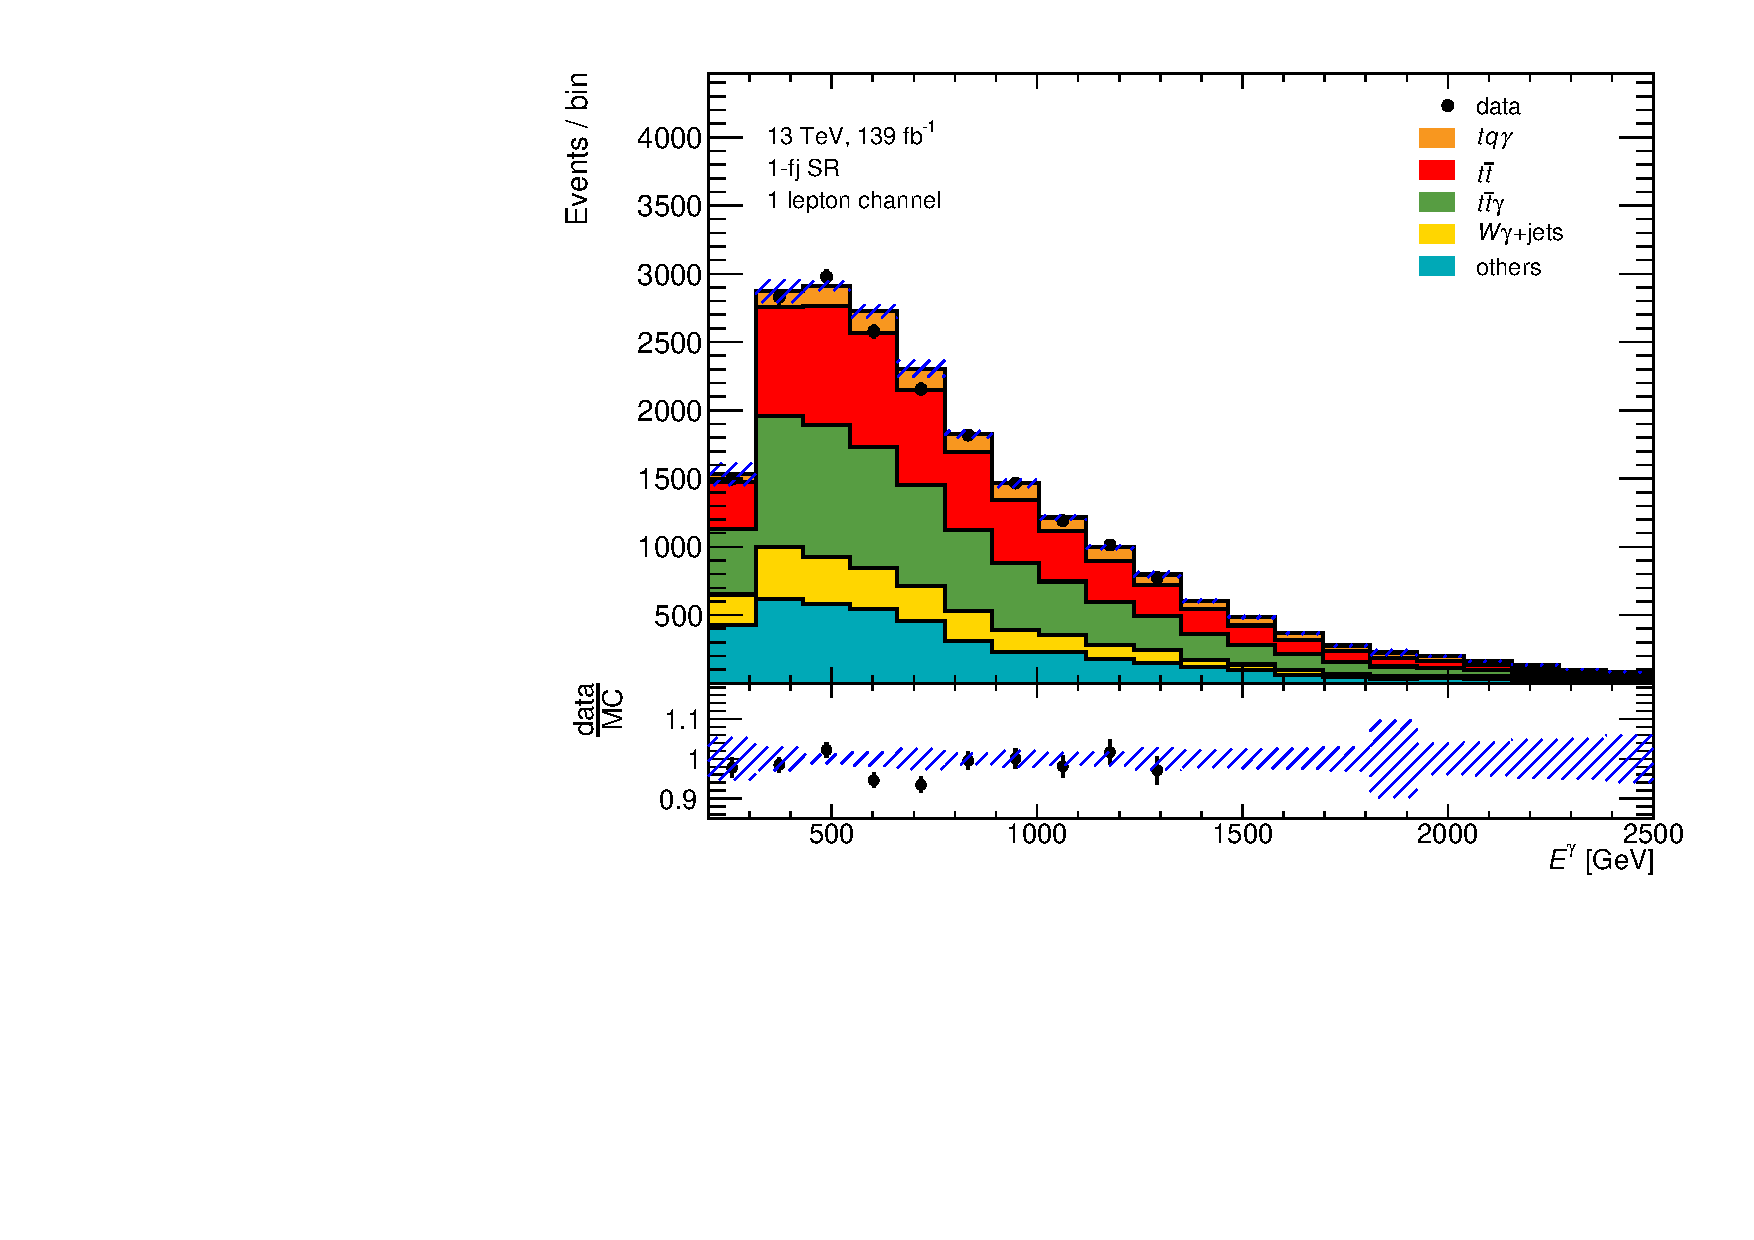
\includegraphics[width=0.7\textwidth]{Plots/fjph_e.pdf}
    \caption{Distribution of the forward jet + photon energy $E_{fj\text{+}\gamma}$.}
    \label{fig:fjph_e}
\end{figure} 

\begin{figure}
    \centering
    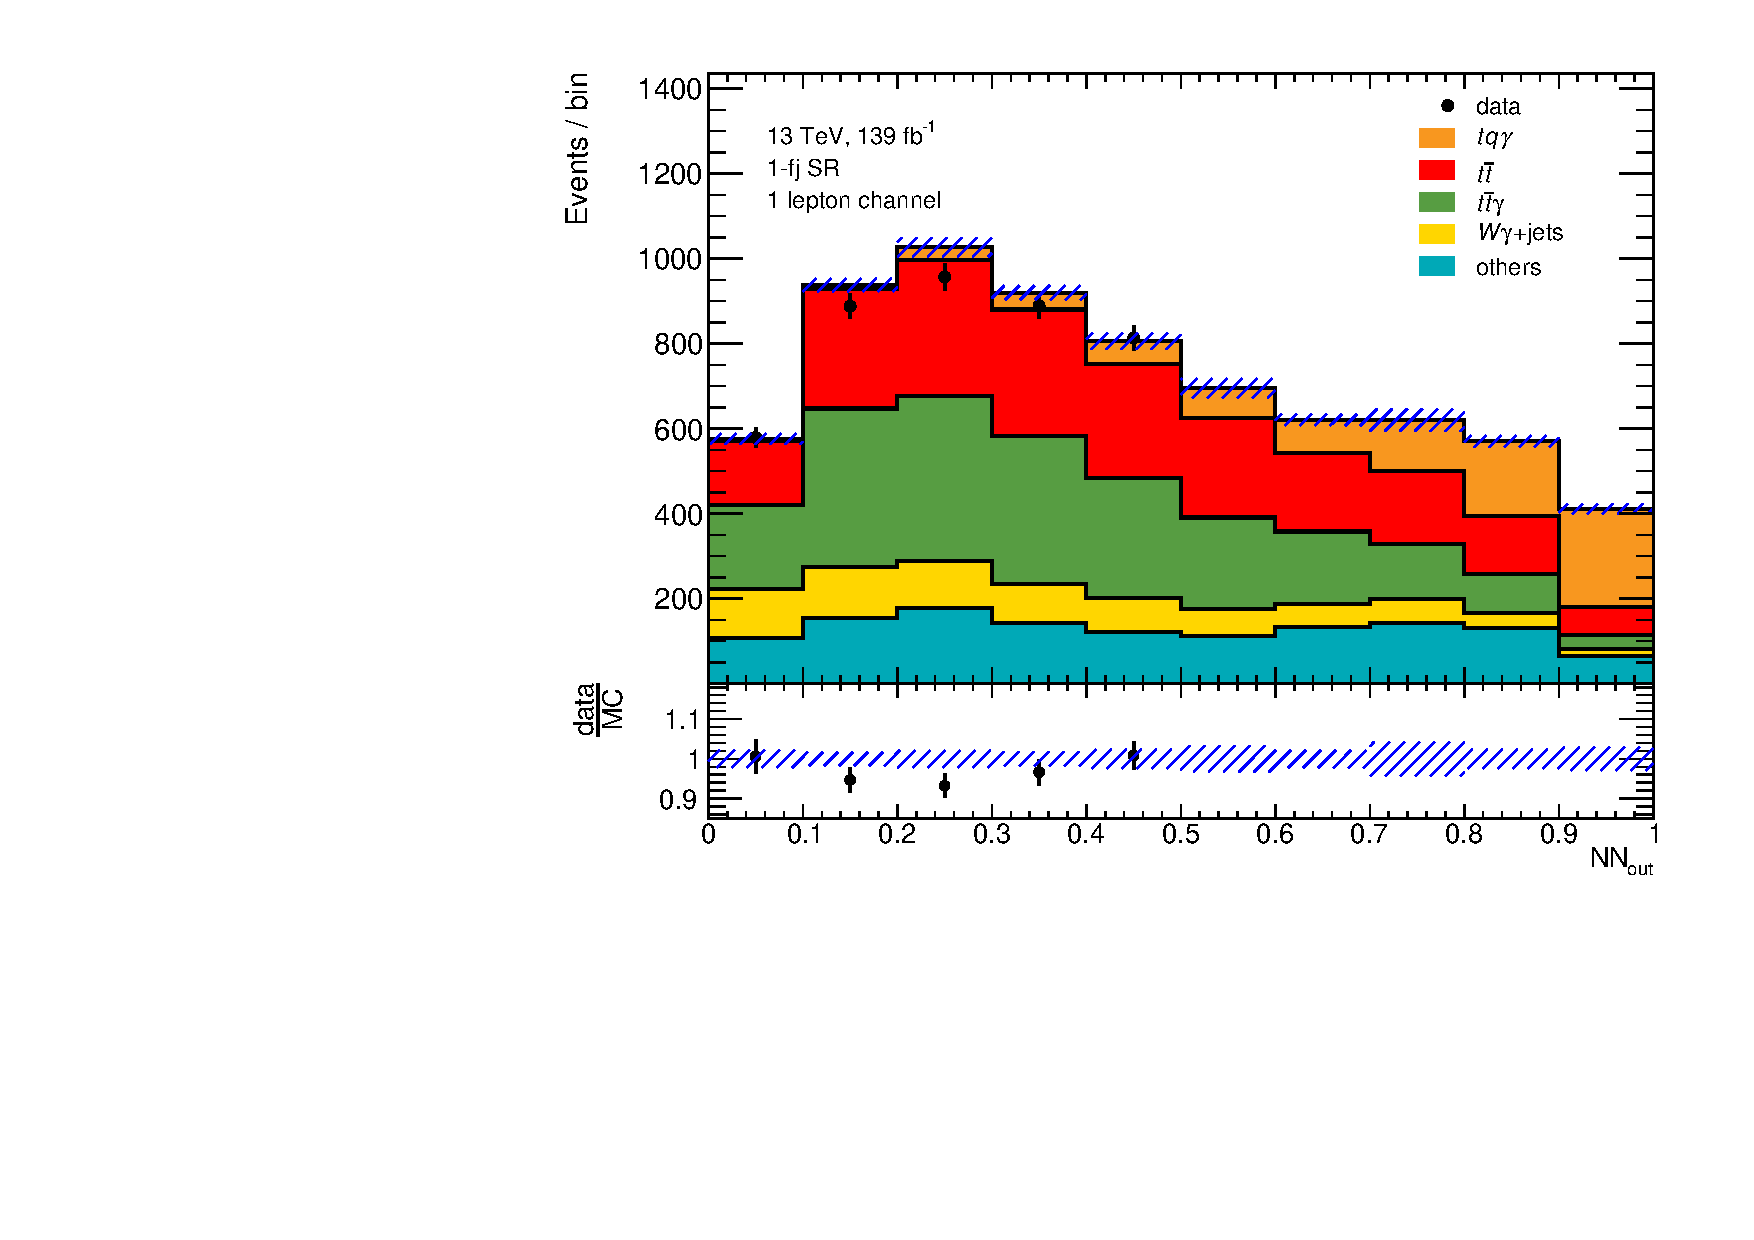
\includegraphics[width=0.7\textwidth]{Plots/NN_out_mixfjphA900.pdf}
    \caption{NN output distribution for the $E_{fj\text{+}\gamma} \geq 900\,\si{\giga\electronvolt}$ region.}
    \label{fig:outputA900fjph_e}
\end{figure} 

\begin{figure}
    \centering
    \begin{subfigure}[b]{0.6\textwidth}
       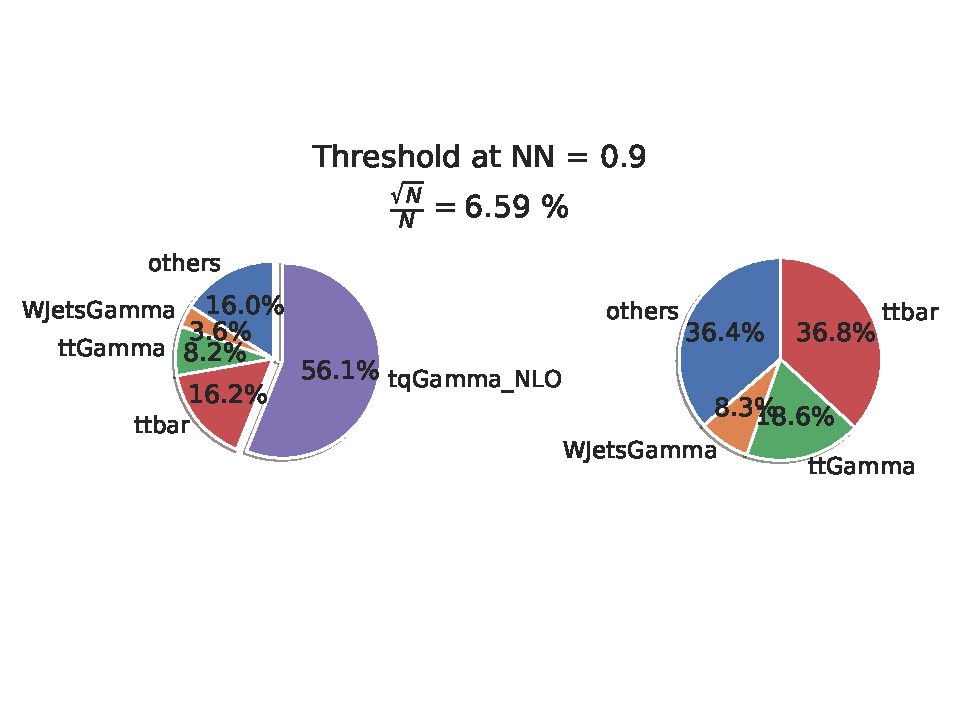
\includegraphics[width=1\linewidth]{Plots/composition9fjA900.pdf}
    \end{subfigure}
    
    \begin{subfigure}[b]{0.6\textwidth}
       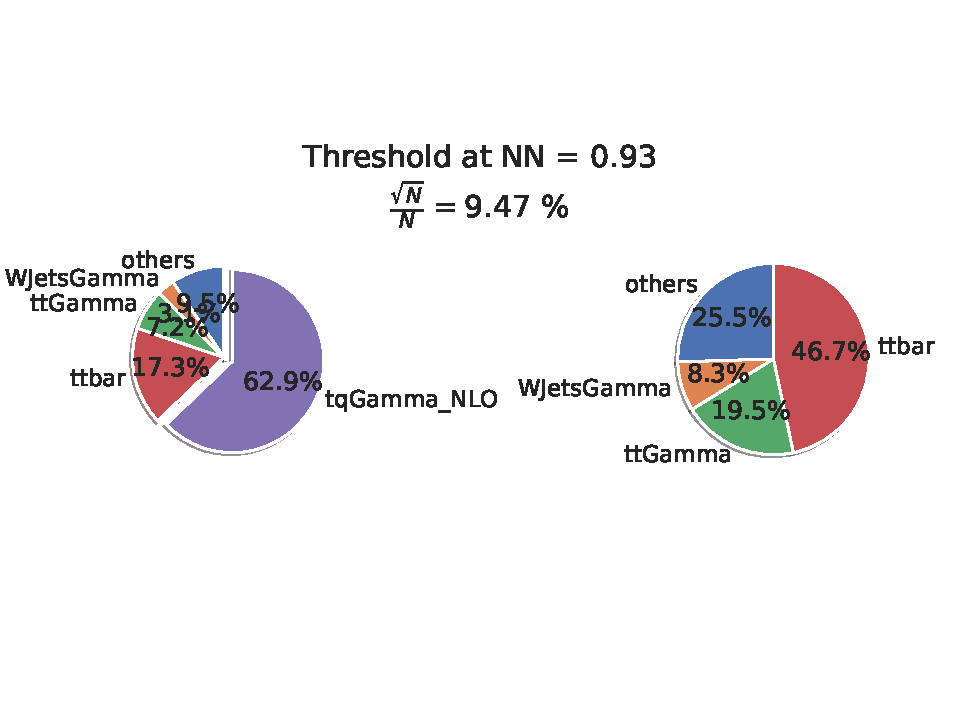
\includegraphics[width=1\linewidth]{Plots/compositionTenphA40.pdf}
    \end{subfigure}
    \caption{Composition of NN output for two different threshholds in the region $E_{fj\text{+}\gamma} \geq 900\,\si{\giga\electronvolt}$. }
    \label{fig:fjph_eA900comp}
\end{figure}